\chapter{مراحل انجام و زمان‌بندی پروژه}
%%%%%%%%%%%%%%%%%%%%%%%%%%%%%%%%%%%%%%%%%%%

با توجه به ویژگی‌هایی که در فصل قبل برای پروژه ذکر کردیم مسیر زیر را برای پیاده سازی پروژه در نظر می‌گیریم \cref{fig.22}.

\begin{figure}[!h]
\centering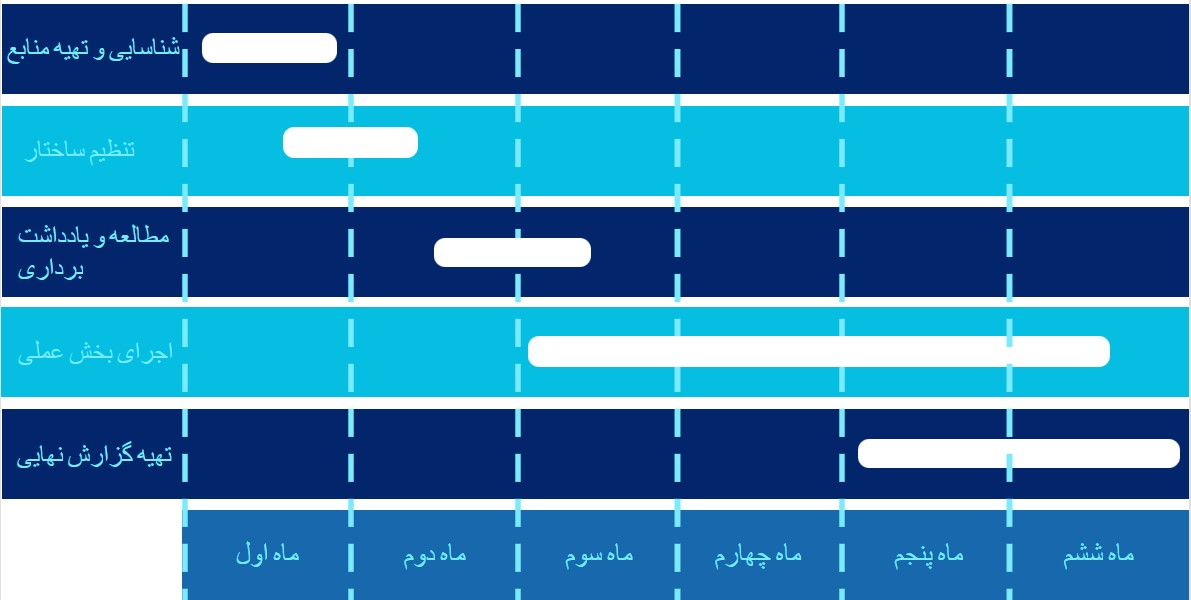
\includegraphics[scale=.55]{./timeline2}
\caption{نمودار زمان‌بندی فعالیت‌ها}\label{fig.22}
\end{figure}
مطالعه و یادداشت برداری شامل موارد زیر خواهد بود:



\begin{itemize}
    \addtolength{\itemindent}{0.6cm}
    \item مطالعه کاملی پیرامون مفهوم مدیریت شبکه‌های کامپیوتری و راه‌های انجام آن
    \item مطالعه کاملی پیرامون پروتکل \lr{SNMP} و پیاده سازی‌های آن
\end{itemize}



همچنین اجرای بخش عملی شامل موارد زیر خواهد بود:



\begin{itemize}
    \addtolength{\itemindent}{0.6cm}
    \item پیاده سازی هسته مدیر \lr{SNMP}
    \item پیاده سازی ماژول ذخیره سازی داده‌های شبکه 
    \item پیاده سازی ماژول کشف شبکه 
    \item پیاده سازی ماژول جمع آوری داده از سطح شبکه 
    \item پیاده سازی ماژول هشدار 
    \item پیاده سازی ماژول پردازش داده‌های شبکه
    \item پیاده سازی یک رابط کاربری در قالب یک وب سایت و ایجاد ارتباط بین ماژول‌های ذکر شده
\end{itemize}
